
%(BEGIN_QUESTION)
% Copyright 2015, Tony R. Kuphaldt, released under the Creative Commons Attribution License (v 1.0)
% This means you may do almost anything with this work of mine, so long as you give me proper credit

Connect a VFD to a three-phase induction motor and to a power cord, in preparation for a set of experiments.  Research the user's manual for the VFD as well as the nameplate on the induction motor to figure out the correct wire connections:

$$\includegraphics[width=15.5cm]{i04295x01.eps}$$

{\it Your instructor will inspect all connections before you apply power!}  Be sure all connections are made through terminal blocks (no taped or twisted wire joints!), and that there are no exposed sections of copper wire for someone to accidently contact!

\vskip 10pt

Next, configure the following parameters in the VFD:

\begin{itemize}
\item{} {\bf ``Base'' parameters} (voltage, frequency, maximum speed, etc.): {\it these values are found on the motor's nameplate, and should always be set \underbar{first} in the VFD before setting any other parameters!  Failure to properly configure the VFD's ``base'' parameters with the motor's nameplate data may result in motor damage!}
\item{} {\bf Acceleration and deceleration times}. {\it Note that you should not set these parameters for unreasonably short times (5 seconds is a good ``minimum'' value), or else you may damage the motor and/or the VFD!}
\end{itemize}

After this, you may try running the motor.  The VFD should provide pushbutton or knob control of the motor's speed, as well as Start and Stop functions.

\vskip 20pt \vbox{\hrule \hbox{\strut \vrule{} {\bf Suggestions for Socratic discussion} \vrule} \hrule}

\begin{itemize}
\item{}  Describe by way of illustration what may happen if the ``base'' parameters within a VFD are set incorrectly, being as specific as possible.
\item{} Some large VFDs need to be ``gently'' powered up if they have been left un-powered for long periods of time, to avoid ``shocking'' the capacitors used to filter their DC busses.  Identify a means of doing so (i.e. limiting the inrush current that will occur when fully discharged capacitors are connected to a voltage source) that is easy and safe to implement.
\item{} Describe a realistic example of how improper ``base'' parameters set in a VFD could cause trouble.
\item{} How should one set the accel and decel times if the goal is to absolutely minimize inrush current?
\item{} Explain why a deceleration time that is too short may result in a VFD {\it DC bus overvoltage} condition.
\item{} How do the accel and decel features of the VFD duplicate the function of a {\it soft-start} unit?
\end{itemize}

\underbar{file i04295}
%(END_QUESTION)





%(BEGIN_ANSWER)


%(END_ANSWER)





%(BEGIN_NOTES)


%INDEX% Final Control Elements, motor: variable frequency drive

%(END_NOTES)


